\section{Formal Methods}
\label{sec:fm}
As the complexity of systems increase, the cost of development and validation consumes more time and resources than ever before; nevertheless, these processes are vital in safety critical systems when the loss of functionality of the system can result in loss of life. Authorities have put in place various thresholds for the likelihood of such events and it is the responsibility of the system developers to show that undesirable events are sufficiently unlikely to occur~\cite{faaSA}. Utilizing the recent advancements in automated formal verification within the validation process has become essential to the certification of critical systems~\cite{deptOfDefense,standard1999,prasad2005survey} and the world of safety analysis began to see its powerful benefits~\cite{hinchey2012industrial, liggesmeyer1998improving, coudert1993fault, Bozzano:2010:DSA:1951720,bozzano2003esacs}. There arose multiple ways of viewing the system and fault models, various ways of automating the capture of safety pertinent information, and a number of tools that addressed practical issues. Formal validation and verification is a proof-based methodology used to assess the correctness of requirements, system design, and implementation. This section provides a background of the formal method techniques that are commonly used in the system development and safety assessment processes.

\subsection{Overview}
Given that this research is focused on model-based system development and safety assessment, we focus our attention onto \emph{model checking} as a method of formal analysis. Model checking is an automatic technique for verifying that system models meet their specified requirements~\cite{clarke2018model}.  Applying model checking to a system design consists of a few main tasks: \emph{modeling}, \emph{formal specification}, and \emph{formal verification}. The digital and mechanical components of a system can be described in abstract form (modeling), and the requirements of the system and of each component can be specified in formal logic (formal specification). Formal verification is demonstrating that the model satisfies its specification using math. The verification of a model takes both the design and the requirement specification into account when analyzing the behavior and interactions of the components. In the sections that follow, we will outline these three major components of model checking and describe the aspects important in this research.

\subsection{Modeling}
\label{sec:modeling}
When modeling a system, the digital and mechanical components are described in abstract form; furthermore, the requirements of the system and of each component can be specified in formal logic. The verification of such models take both the architecture and the requirement specification into account when analyzing the behavior and interactions of the components comprising the system. Throughout the past few decades, numerous modeling languages and tools have been introduced, for example Simulink from MathWorks~\cite{MathWorks}, SCADE from Esterel Technologies~\cite{abdulla2004designing}, and research base languages such as Lustre~\cite{Halbwachs91:IEEE}. Other common modeling languages include SysML~\cite{friedenthal2014practical} and AADL~\cite{FeilerModelBasedEngineering2012}. 

Often, engineers who design safety critical systems model their systems as networks of operators transforming flows of data. At a higher level, this can be represented by block diagrams that group these networks into reusable components. {\em Dataflow} languages allow these models to directly represent the digital control system. Dataflow programming languages have several merits, one of which is that the program is a completely functional model of the system. This feature makes the model well suited to formal verification and program transformation; it also facilitates reuse, because the module will behave the same way in any context into which it is embedded~\cite{joshi2008behavioral}. For this dissertation, we focus our attention on Lustre~\cite{Halbwachs91:IEEE}, a synchronous\footnote{A synchronous language breaks real time into a sequence of instants in which the outputs of the model are computed.} dataflow programming language used in the formal verification portion of this research. Lustre is described in more detail in Section~\ref{sec:lustre}. 




\begin{comment}
\subsubsection{Ordered Binary Decision Diagrams}
A Binary Decision Diagram (BDD) is a data structure used to encode Boolean formulae.
\begin{figure}[htbp]
        \center{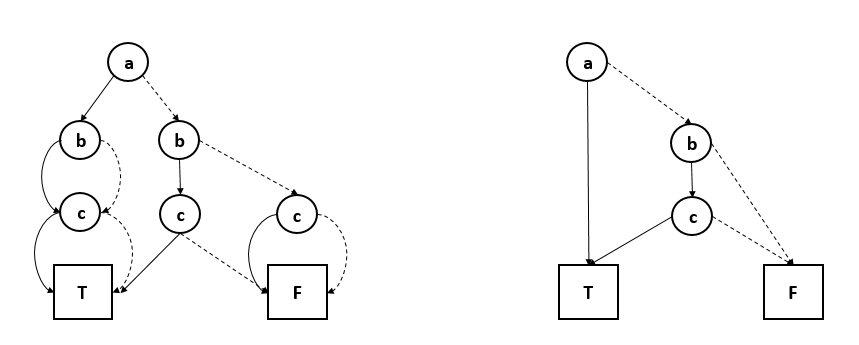
\includegraphics[width=0.8\textwidth] {images/bdd.png}}
        \caption{\label{fig:bdd} Binary Decision Diagrams of the Formula $a \lor (b \land c)$}
\end{figure}
As shown in Figure~\ref{fig:bdd}, it is a rooted, directed, acyclic graph with internal decision nodes and two terminal nodes (\textit{true} and \textit{false}). Each of the decision nodes is labeled with a Boolean variable and has two child nodes, low child and high child. The edge from a node to its low child represents the assignment of \textit{false}, likewise the edge to the high child represents the assignment of \textit{true}. The BDD is called \textit{ordered} if different variables appear in the same order on all paths from the root. Intuitively, following a path from the root to the \textit{true} terminal node represents a valid assignment to the Boolean formula (invalid in the case of ending on the \textit{false} terminal node). 

BDDs are reduced by the removal of isomorphic subgraphs. The BDD shown on the right of Figure~\ref{fig:bdd} is the reduced form of the BDD on the left.
\end{comment}


\subsection{Formal Specification}
\label{sec:formalSpec}
Before we can verify the correctness of a system, we must first specify the properties that the system should have~\cite{clarke2018model}. The formal specification process translates the informal system requirements into a mathematical logic to determine if the system design is correct~\cite{hinchey2012industrial}. This process guarantees an unambiguous description of the requirements, which is not possible when using an informal natural language. The formal definition of system requirements includes the system design and its expected behavior as well as the assumptions on the environment in which the system is expected to operate. A design or implementation can never be considered correct in isolation; it is only correct with respect to the specifications. The expected behavior, system design, and environmental assumptions change and are refined as the system goes through the various stages of development~\cite{lamsweerde2000formal}. A commonly used method of specification is \emph{temporal logic}. Temporal logics are useful for specifying complex system requirementss, because they can describe the ordering of events in time without introducing time explicitly. 

\subsubsection{Linear Temporal Logic}
Temporal logic can be used to express properties of reactive systems~\cite{Bozzano:2010:DSA:1951720}. System properties are usually classified into two main categories: {\em safety properties} and {\em liveness properties}. Safety properties express the idea that ``nothing bad ever happens" where liveness properties state that ``something good will eventually happen." 

An example of a safety property is: ``it is never the case that the brake pedal is pressed and no hydraulic pressure is supplied at the wheel." A liveness property, on the other hand, could state: ``eventually the process will complete its execution." 

Traditionally, two types of temporal logic are used in model checking; Computational Tree Logic (CTL), which is based on a branching time logic model, and Linear Temporal Logic (LTL), based on a linear representation of time. This research will focus on LTL. 

An LTL formula is built from a set of atomic propositions, logical operators, and basic temporal operators. The formula is evaluated over a linear path or sequence of states, $s_0, s_1, ..., s_i ,s_{i+1},...$. The following temporal operators are provided:
\begin{itemize}
    \item Globally (\textbf{G}): $G_p$ is true in a state $s_i$ if and only if $p$ is true in all states $s_j$ with $j \geq i$.
    
    \item Finally (\textbf{F}): $F_p$ is true in state $s_i$ if and only if $p$ is true in some state $s_j$ with $j \geq i$.
    
    \item Next (\textbf{X}): $X_p$ is true in state $s_i$ if and only if $p$ is true in the state $s_{i+1}$. 
    
    \item Until (\textbf{U}): $pUq$ is true in state $s_i$ if and only if $q$ is true in some state $s_j$ with $j \geq i$ and $p$ is true in all states $s_k$ such that $i \leq k < j$.
\end{itemize}

Other temporal operators can be defined on the basis of the operators above~\cite{sistla1985complexity}. Formal definitions and more information on LTL and CTL can be found in a number of research works~\cite{Bozzano:2010:DSA:1951720, clarke2018model}.

\subsection{Formal Verification} 
\label{sec:formalVer}
Once we have specified the important properties (formal specification), then a formal model for the system is created; this model captures the properties that must be considered to establish correctness~\cite{clarke2018model}; this process is referred in this dissertation as \emph{formal verification}. Formal verification is the use of proof methods to show that given the environmental assumptions stated in the formal specification, the formal design of the system meets the requirements. The problem can be reduced to that of property checking: given a program $P$ and a specific property, does the program satisfy the given property~\cite{fitting2012first}.  

Model checking was introduced in the early 1980s and consists of exploring the states and transitions of a model~\cite{clarke1981design,queille1982specification}. By representing the system abstractly, a possibly infinite state space is reduced to a finite model.~\cite{d2008survey}. The proofs are generated over an abstract mathematical model of the system, such as finite state machines, labeled transition systems, or timed automata. It takes as input a model of a system and the properties written in formal logic, then explores the state space of the system to determine if the model violates the properties~\cite{clarke2018model,fraser2009testing}. In recent years, model checking takes advantage of abstraction techniques specific to a domain to consider multiple states or transitions in a single operation; this lessens computation time considerably~\cite{d2008survey}. Nevertheless, the biggest limiting factor of model checking is scalability and much of the recent research in this area attempts to address this problem~\cite{clarke2018model}.

Deductive methods of verification consists of generating proof obligations from the specifications of the system and using these obligations in a theorem prover setting. Automated theorem provers have the main objective to show that some statement (conjecture) is a logical consequence of other statements (the axioms and hypotheses). The rules of inference are given as are the set of axioms and hypotheses~\cite{d2008survey,fitting2012first}. Deductive methods of verification include automated theorem provers (e.g., Coq~\cite{coq}, Isabelle~\cite{isabelle}) and satisfiability modulo theories (e.g., SMTInterpol~\cite{smtInterpol}, Z3~\cite{z3}, Yices~\cite{yices}). 


